% Cuerpo del documento
\subsection*{Introducción}
En los últimos años, el correcto uso de los recursos hidráulicos se ha convertido en tema de interés. Esto se debe principalmente a la cada vez más notable escasez de agua potable, tanto por acción del cambio climático, como por el creciente uso indiscriminado de este recurso para satisfacer las crecientes necesidades de la población y al prácticamente nulo tratamiento de las aguas residuales \emph{\citep{informeods2021, aa2030}}.\\
Según datos del Sistema de Información del Agua (SINA), para 2021 el número de plantas en activo aumento a 2872, de las cuales, 818 utilizan el sistema de lodos activados con un caudal de agua tratada de 106.603 m$^{3}$/s, siendo un 73\% del caudal que recibe un tratamiento, seguido de las lagunas aireadas con un 10.3\%, los filtros biológicos con el 3.8\%, entre otros \emph{\citep{SINA}}.\\
La Comisión Estatal del Agua (CEA), que es la institución encargada del vigilar el uso correcto del agua en el estado de Jalisco, mediante la ficha técnica hidrológica del municipio de Lagos de Moreno, informa que se cuentan con 3 plantas de tratamiento de aguas residuales  en funcionamiento con capacidad de operación de 114.6 L/s, cubriendo un 33.8\% de saneamiento (datos pertenecientes al 2015) \emph{\citep{fichalagos}}. De las tres plantas que se encuentran en operación, todas utilizan el proceso de lodos activados convencional, las cuales son: planta Paso de Cuarenta, con un caudal medio de operación de 9 L/s; planta Parque Industrial, con un caudal de operación de 2 L/s; y finalmente la planta municipal (en la cual se basa la presente investigación), ubicada a las afueras de la zona urbana de Lagos de Moreno a margenes del río Lagos con un caudal promedio de 104 L/s \emph{\citep{fichalagos}}.
\subsection*{Antecedentes}
\subsubsection*{Aguas Residuales}
Podemos definir a las aguas residuales como aquellas que provienen de las actividades del hombre y de los animales, tanto como de las precipitaciones, y que son recolectadas en los sistemas de alcantarillado o vertidas directamente al ambiente \emph{\citep{carreno17}}.
\subsubsection*{Clasificación de las aguas residuales}
Podemos dividirlas según su origen en dos clases importantes:
\begin{description}
\item[\textit{Aguas residuales domésticas}]
Las aguas residuales domésticas son flujos de agua conformados por la combinación de las excretas eliminadas por la población, que incluye heces y orina; además, contiene desechos de animales domésticos, residuos de lavandería, residuos de industrias caseras. La gente excreta de 100 a 500 g de heces por día y de 1 a 3 L de orina al día, contribuyendo con una DBO$_{5}$ de 20 a 45 g por día \emph{\citep{carreno17}}. 
\item[\textit{Aguas residuales municipales}]
Son aquellas provenientes tanto de los efluentes domésticos como de las pequeñas industrias y otras actividades realizadas en las áreas urbanas (comercios, oficinas, restaurantes, mercados de abasto, etc.) y que incrementan los contaminantes con algunos componentes que pueden resultar indeseables para los tratamientos convencionales \emph{\citep{carreno17}}.
\end{description}

\subsubsection*{Tratamiento de aguas residuales}
El tratamiento de aguas residuales, es un servicio que consiste en la separación de la carga orgánica que contienen las aguas residuales, eliminando al máximo la cantidad de residuos y contaminantes, siendo algunos de los más importantes los descritos en el Cuadro~\ref{tab:constituyentes} \emph{\citep{tratGOB, ron}}, de tal forma que reúnan los requisitos de calidad que permiten las normas legales y regulaciones de cada país, con la finalidad de que los estándares de calidad ambiental (\emph{ECA}) permanezcan inalterables en el tiempo, y que la preservación sustentable de los ecosistemas sea posible. Sin embargo, en los países en desarrollo esto no se cumple, por lo que solo un pequeño porcentaje de aguas residuales tienen tratamiento y el resto son vertidas al mar, ríos, suelos, etc., originando riesgos de infecciones gastrointestinales de origen hídrico \emph{\citep{carreno17}}.\\
	\begin{table}[!ht]
	\caption{Principales constituyentes de interés en el tratamiento de aguas residuales}\label{tab:constituyentes}
	\begin{center}
		\begin{tiny}
		\begin{tabular}{ | m{5cm} | m{10cm} | }
		\hline
		\rowcolor{blanc}
		{\textbf{Constituyentes}} & {\textbf{Razones de interés}}\\ 
		\hline 
		Sólidos suspendidos totales & Formación de depósitos de lodos y condiciones anaerobias\par \\ 
		
		Compuestos orgánicos biodegradables & Agotamiento del oxígeno en fuentes naturales y desarrollo de condiciones sépticas\par \\
		
		Constituyentes inorgánicos disueltos (p.ej. sólidos disueltos totales) & Constituyentes inorgánicos adicionados por el uso. Aplicaciones en el reciclaje y en la reutilización de aguas residuales\par \\
		
		Metales pesados & Constituyentes metálicos adicionados por el uso. Muchos se clasifican como polulantes de prioridad\par \\
		
		Nutrientes & Crecimiento excesivo de la vida acuática indeseable, eutroficación, concentración de nitratos en agua para consumo\par \\
		
		Patógenos & Trasmisión de enfermedades\par \\
		
		Contaminantes orgánicos prioritarios & Sospechosos de ser carcinogénicos, mutagénicos, teratogénicos o de toxicidad aguda alta. Muchos de los polulantes prioritarios son resistentes a los métodos de tratamiento convencionales (conocidos como compuestos orgánicos refractarios)\\
		\hline
		\end{tabular}
		{\small{Fuente: Crites y Tchobanoglous (2000)}}
		\end{tiny}
	\end{center}
	\end{table}
El problema de cálculo, diseño y operación, empieza a complicarse en el intento de eliminar las sustancias orgánicas putrescibles, ya disueltas, o en forma coloidal por biodegradación, presentando la mayor dificultad en la etapa de tratamiento secundario, donde se logra hacer desaparecer la contaminación de las aguas \emph{\citep{ron}}.\\
Un sistema de tratamiento secundario de aguas residuales cuanta con un reactor biológico al que le llegan las corrientes procedentes de la etapa de tratamiento primario y la de retorno de lodos, a la vez que se suministra oxígeno al sistema mediante aireación. De modo que el sustrato orgánico es biodegradado por los lodos activos, generándose nueva masa de lodos activos. El contenido del reactor biológico fluye al sedimentador secundario, también llamado clarificador final, en donde se separa una corriente superior clarificada, que pasa a tratamiento terciario. La corriente inferior del sedimentador, constituida por lodos activos concentrados, retorna un caudal de reciclaje de lodos \emph{Q$_{r}$}, en su mayor parte del reactor biológico, y una pequeña fracción, conocida como caudal de desecho \emph{Q$_{w}$}, se lleva fuera de esta etapa para su tratamiento específico posterior (\emph{ver} Figura~\ref{fig:balance}) \emph{\citep{manuel13}}.
	\begin{figure}[!h]
		\centering
		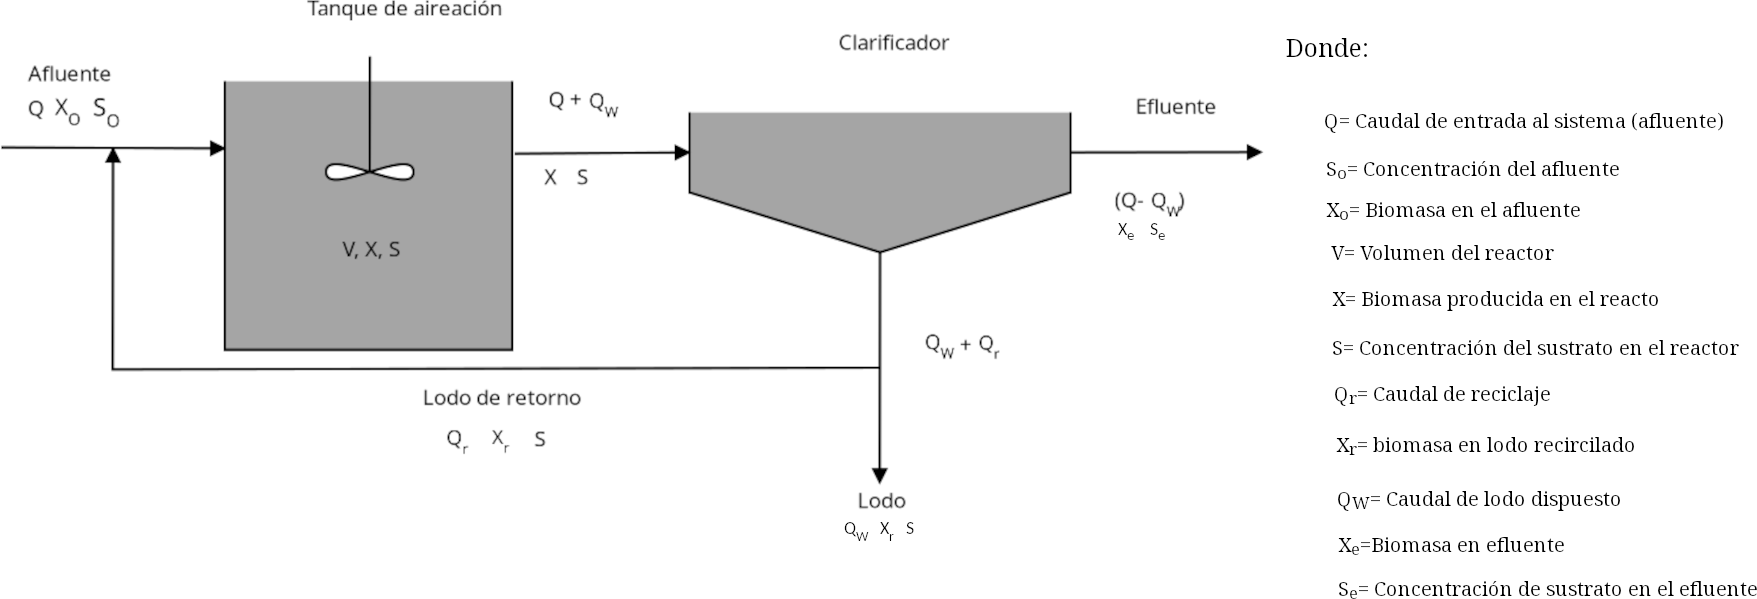
\includegraphics[scale=0.52]{Diagrama_de_flujo.png}
		\caption{Tratamiento secundario de Aguas Residuales}
		\small{Fuente: Elaboración propia}
		\label{fig:balance}
	\end{figure}
\subsubsection*{Lodos activados}
El tratamiento con lodos activados es un proceso de tratamiento biológico que involucra cultivo en suspensión de microorganismos aeróbicos, con el fin de degradar los contaminantes presentes en el afluente. El cultivo se lleva a cabo en condiciones de mezclado tanto por movimiento mecánico, utilizando propelas y difusores; como por el uso de aereadores que permitan la unión de todos los componentes del caldo de cultivo. Una serie de reacciones bioquímicas tienen lugar en los tanques de aireación, en las cuales se degradan los componentes orgánicos para generar nuevos componentes celulares \emph{\citep{ashok16}}.\\
	\begin{figure}[!h]
		\centering
		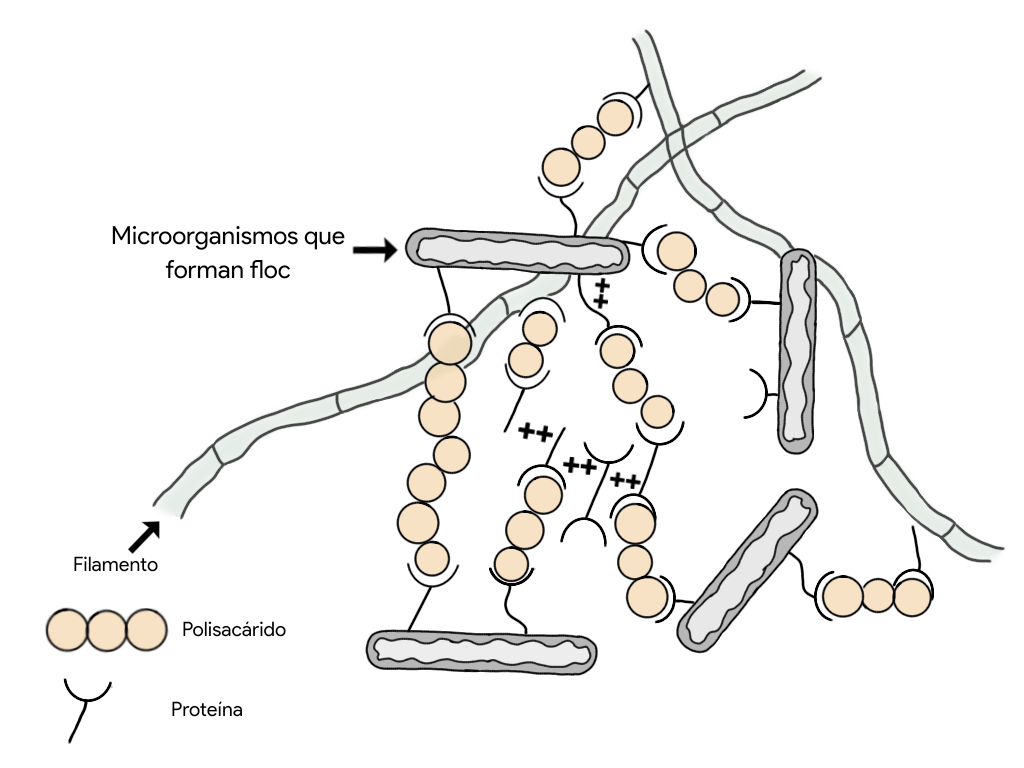
\includegraphics[scale=0.15]{Floculo.png}
		\caption{Modelo de formación de los flocs en lodos activados propuesto por Higgins (1997)}
		\small{Fuente: Elaboración propia}
		\label{fig:modfloc}
	\end{figure}
La unidad ecológica de los lodos es el flóculo individual. Los flóculos de los lodos son cúmulos de varios millones de células bacterianas (principalmente cepas gram-negativas), junto con algunos otros organismos como: hongos, protozoos, rotíferos y nematodos; y materias inertes, orgánicas e inorgánicas (Figura~\ref{fig:modfloc}). La naturaleza floculenta de los lodos activados resulta importante, en primer lugar para la absorción de las materias coloidales, iónicas y en suspensión dentro del agua residual, y en segundo lugar para la separación rápida, eficiente y económica de la masa microbiana del agua residual tratada~\emph{\citep{ashok16}}.\\ 
Al airear un agua residual que contenga nutrientes orgánicos tenderá a desarrollar un lodo procedente de los microorganismos ya presentes en ella, o que han entrado de la atmósfera. El proceso de desarrollo de los lodos se puede acelerar por una siembra con una población microbiana, como lodos procedentes de otro proceso, tierras, o en el caso de un desecho industrial que contenga nutrientes fuera de lo común, un cultivo especialmente desarrollado en el laboratorio o una planta piloto~\emph{\citep{winkler96}}.
Con el paso de los años se han desarrollado variaciones del proceso de lodos activados. Los procesos principales de lodos activados se pueden clasificar como lo muestra la Figura~\ref{fig:procesosaer}.\\
	\begin{figure}[!h]
		\centering
		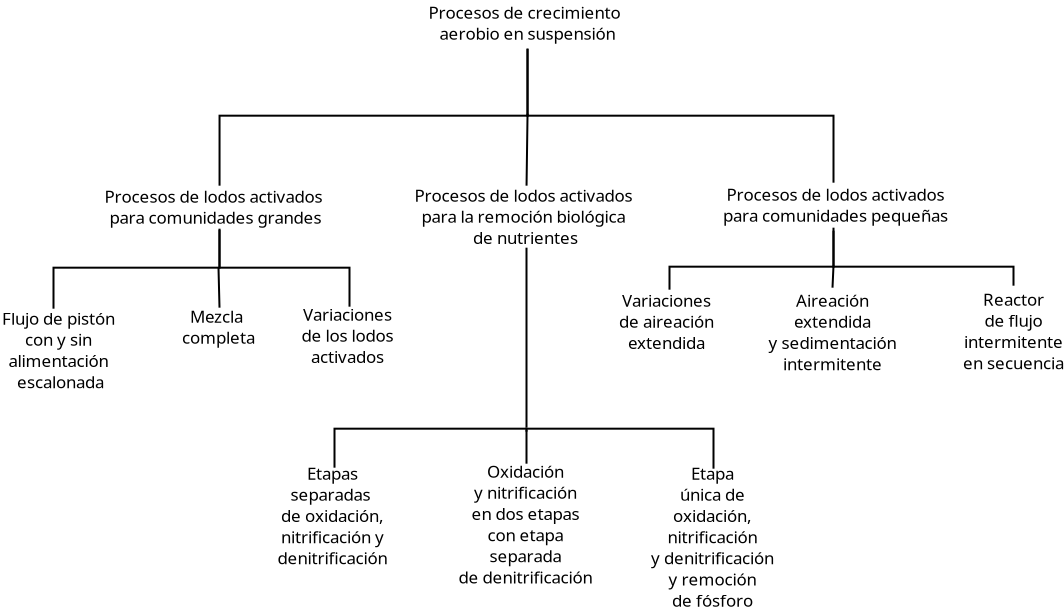
\includegraphics[scale=0.2]{Clasificacion_procesos_aer.png}
		\caption{Esquema de clasificación de los procesos de lodos activados}
		\small{Fuente: Crites (2000)}
		\label{fig:procesosaer}
	\end{figure}
La temperatura, el pH y el potencial de óxido-reducción son otros de los factores que juegan un papel importante si se busca que el proceso de lodos activos se lleve a cabo de manera efectiva. El rango optimo de pH se encuentra entre 6.5 y 9.0; si el pH esta por debajo de 6.5 los hongos podrían por sustrato por encima de las poblaciones bacterianas. El rol que tienen las bacterias en el proceso de lodos activos se muestra de manera detallada en la Figura~\ref{fig:rolbacteria}~\emph{\citep{ashok16, winkler96}}.
	\begin{figure}[h]
		\centering
		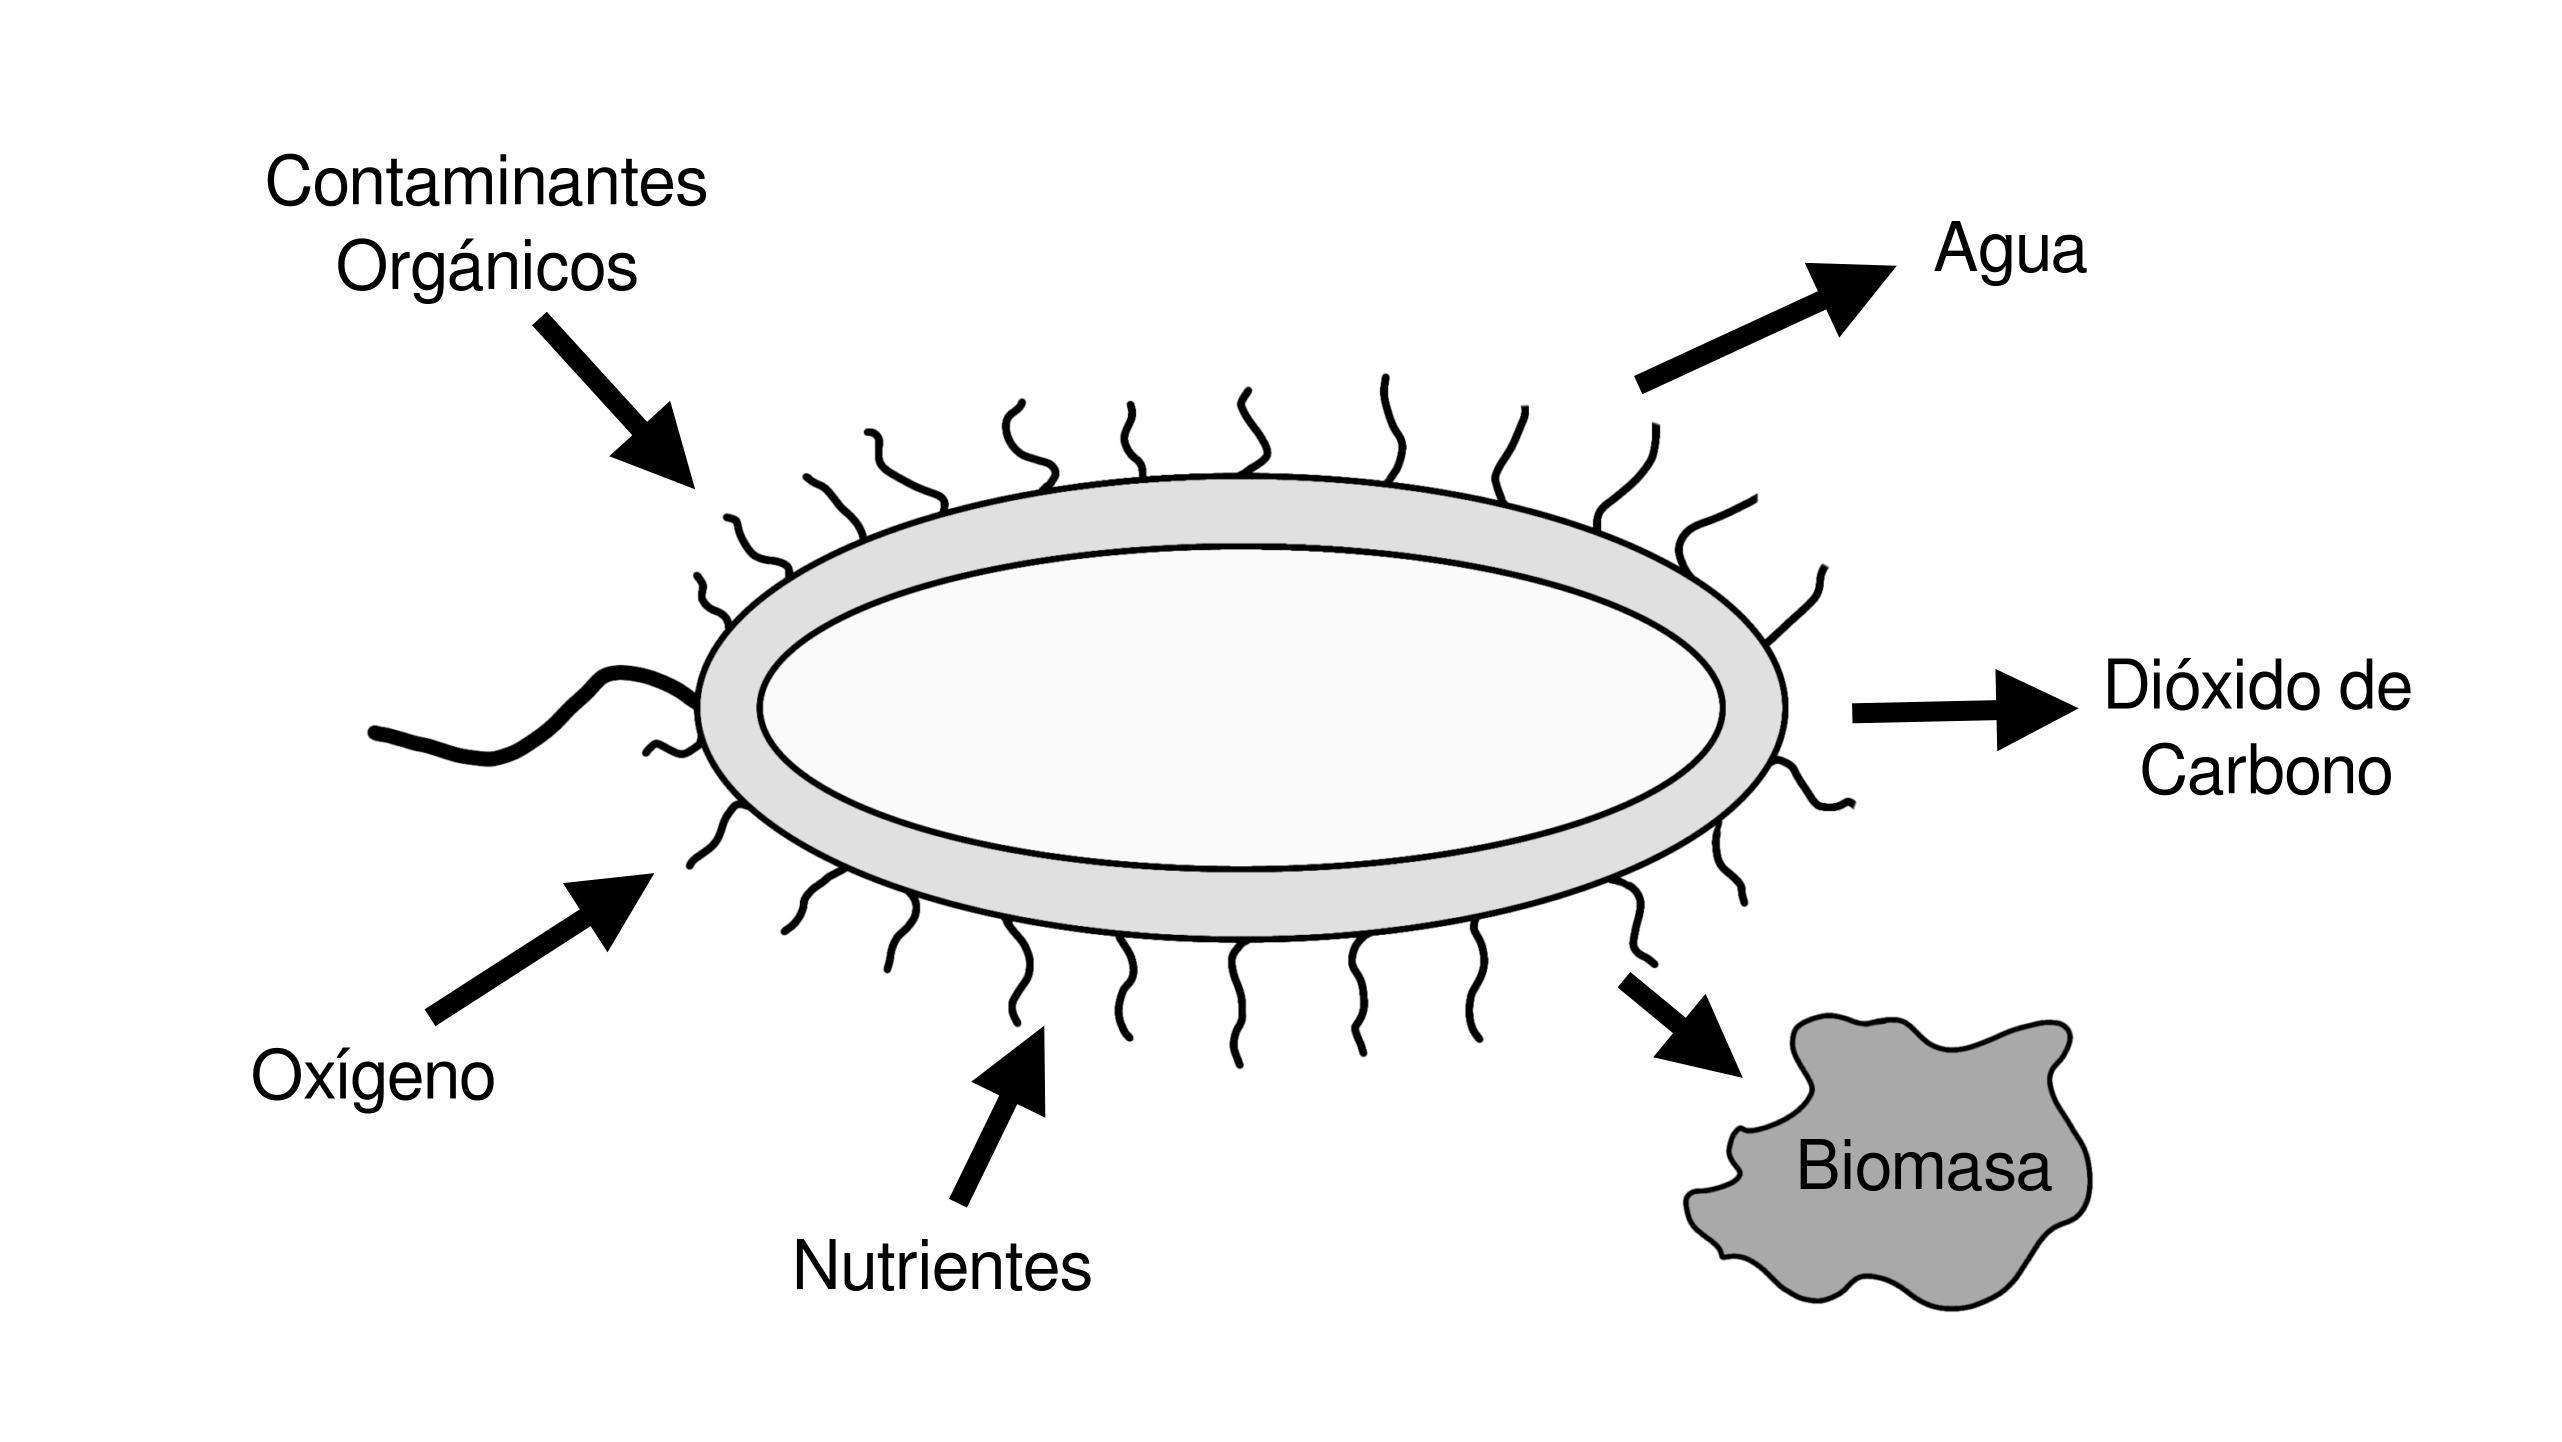
\includegraphics[height=3.5cm,width=8.5cm]{Bacteria_rol.png}
		\caption{Proceso metabólico bacteriano durante el proceso de lodos activados}
		\small{Fuente: Rathoure (2016)}
		\label{fig:rolbacteria}
	\end{figure}
\subsubsection*{Parámetros de crecimiento de lodos}
Los parámetros biocinéticos manifiestan el comportamiento de los lodos activados al desarrollarse en determinada agua residual. Con base a estos, se pueden obtener por ejemplo: la carga de oxígeno (kg/d) que los lodos biológicos requieren para oxidar la materia orgánica presente; los kilogramos de lodos producidos por la oxidación de la materia orgánica contaminante; las constantes de velocidad; de remoción de contaminantes; de crecimiento; igualmente, a partir de esos parámetros, podemos conocer otros datos importantes con relación a la ingeniería básica del sistema de tratamiento, como lo son: los tiempos de residencia en el biorreactor; el volumen del biorreactor; la capacidad del sistema de aireación; la recirculación de lodos al biorreactor; la carga de lodos que es preciso desechar, etc \emph{\citep{martinez2005}}.
	\begin{figure}[!h]
		\begin{center}
		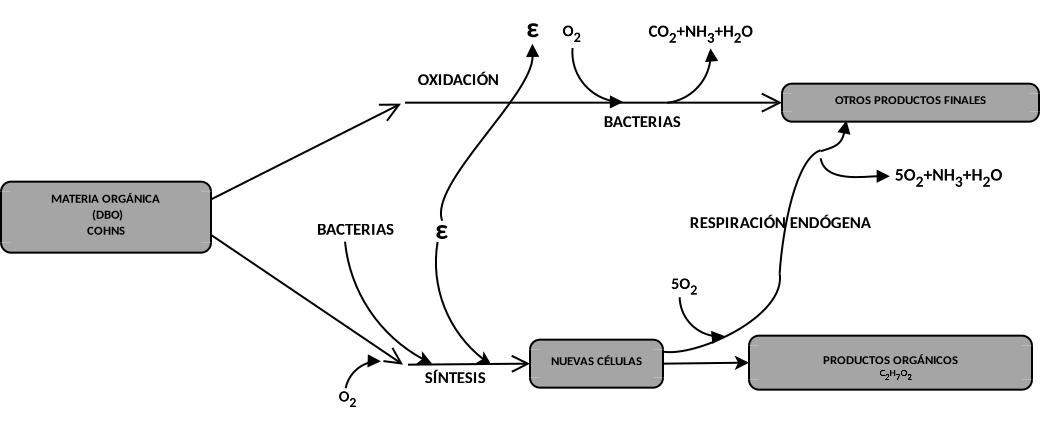
\includegraphics[scale=0.25]{Estabilizacion_mat_org.png}
		\caption{Estabilización de la materia orgánica (DBO) con formación de células nuevas y productos finales}
		\small{Fuente: Crites (2000)}
		\label{fig:estabilizacion}
		\end{center}
	\end{figure}
\\Los microorganismos degradan la materia orgánica soluble en el agua residual siguiendo una cinética específica de remoción de materia orgánica, expresada como remoción de la DBO soluble (\emph{véase} Figura~\ref{fig:estabilizacion}); otras veces puede expresarse como DQO soluble. Entre los modelos más comunes de cinética de remoción de DBO soluble, se encuentran el modelo de \textbf{primer orden}, el de \textbf{orden variable} o \textbf{Monod}, y el de \textbf{Grau}. Los datos experimentales que se obtengan, se utilizan para ajustar un modelo de cinética de remoción, que puede estar entre los anteriormente señalados; de no ser así, se tendrá que probar con otros reportados en bibliografía; incluso, podría ser necesario generar un modelo propio (\emph{ver} Figura \ref{fig:ecuaciones})~\emph{\citep{martinez2005}}.\\ \\ \\
	\begin{figure}[!h]
		\centering
		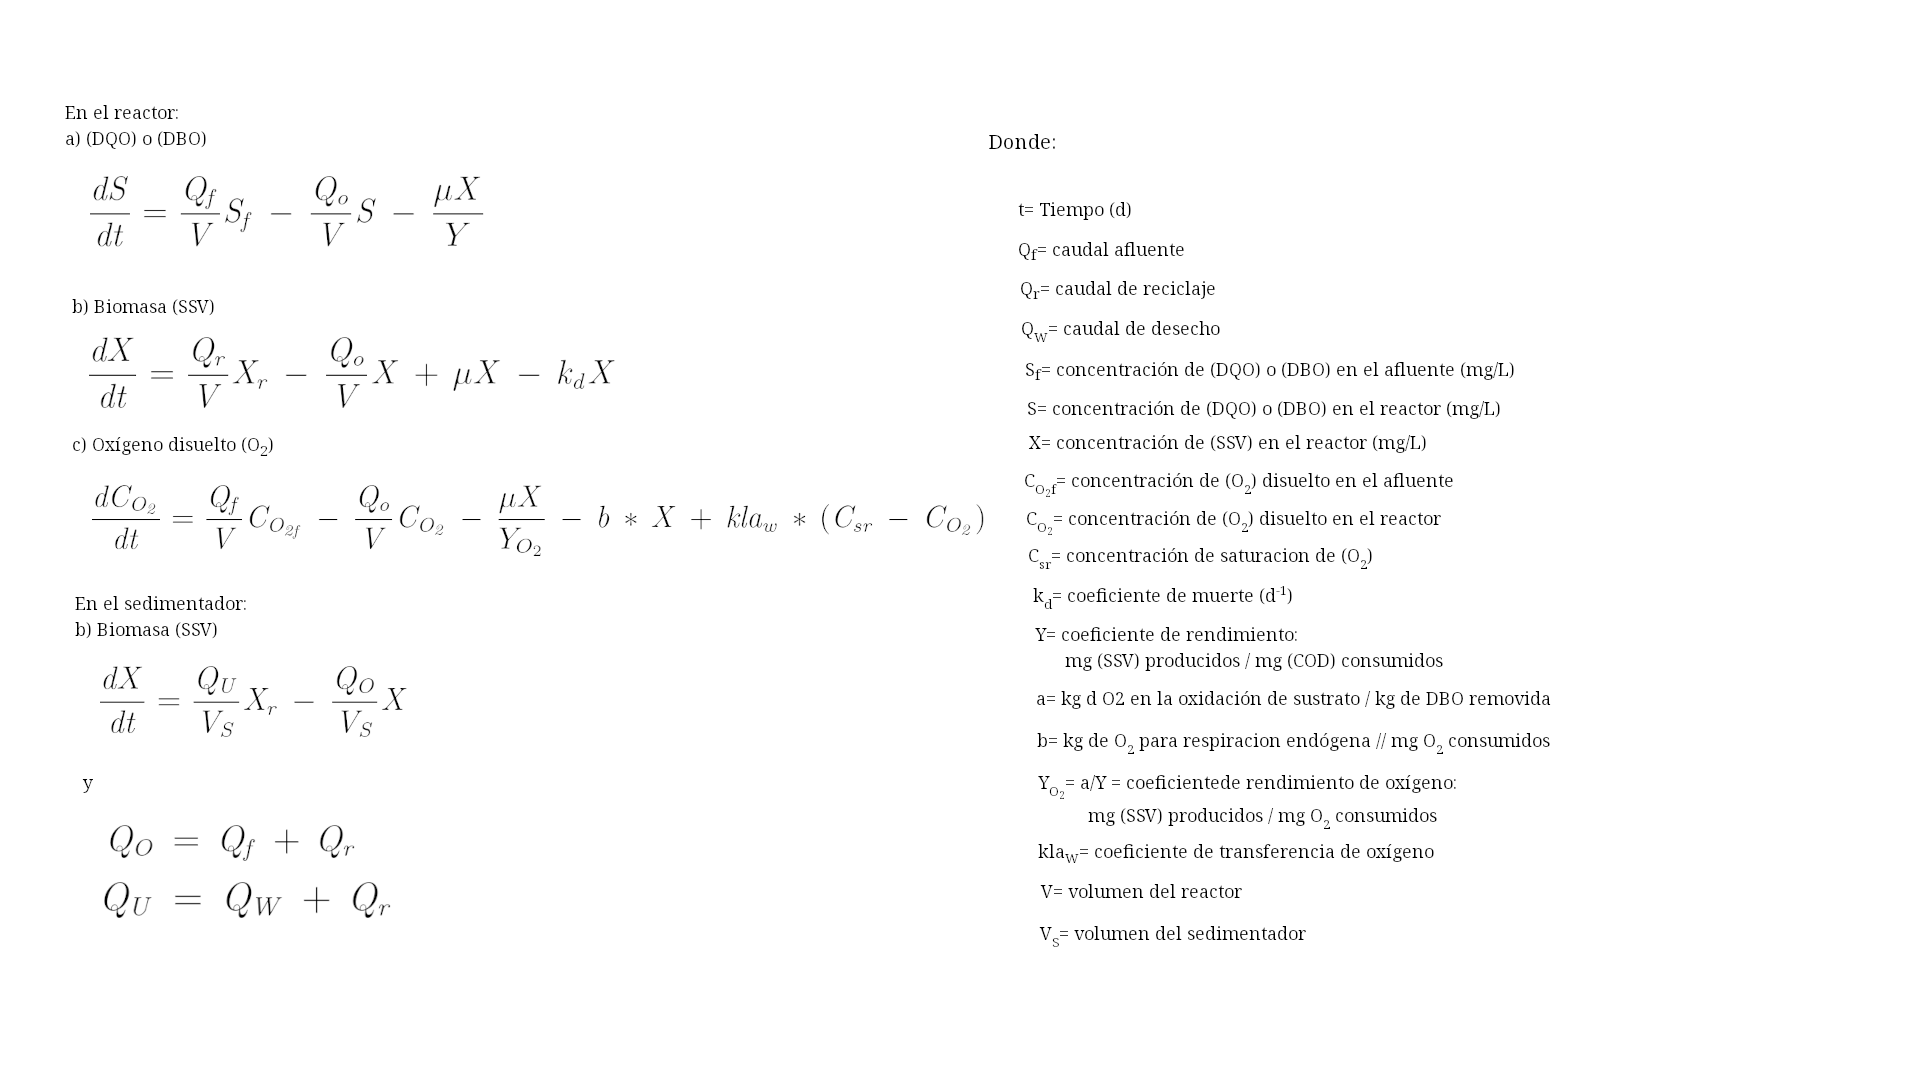
\includegraphics[scale=0.4]{Ecuaciones.png}
		\caption{Balances en el sistema de tratamiento de lodos}
		\label{fig:ecuaciones}
		\small{Fuente: Martínez (2015)}
	\end{figure}
\\Los principales ensayos para determinar la carga orgánica de un desagüe son: 
\subsubsection*{Oxígeno disuelto (OD)}
La cantidad de oxígeno presente en las plantas de tratamiento de aguas residuales (PTAR) determina sus condiciones aerobias, microaerófias, anóxicas y anaerobias para los procesos biológicos. Los desagües crudos, generalmente tienen bajas concentraciones de OD, mientras que los desagües sépticos son anaeróbicos; para los procesos de desnitrificación es necesario un ambiente anóxico, es decir no necesariamente anaeróbico estricto; mientras que en los tanques de aireación de lodos activados y las lagunas aireadas es necesaria la incorporación de oxígeno al sistema \emph{\citep{carreno17}}.
\subsubsection*{Demanda bioquímica de oxígeno (DBO)}
Se define como la cantidad de OD consumido por los microorganismos para la oxidación de la materia orgánica carbonácea (DBO carbonácea). Puede considerarse como un procedimiento en el cual los organismos vivos sirven como medio para la oxidación de la materia orgánica hasta dióxido de carbono y agua~\emph{\citep{carreno17}}.\\
Las reacciones bioquímicas de esta actividad metabólica se resumen en reacciones de síntesis de nuevos organismos, reacciones de producción de energía, para desarrollo de su actividad y reacciones de degradación de los propios microorganismos, consumiendo estas tres reacciones oxígeno, hasta que el sustrato disponible se agota, comenzando entonces la fase de metabolismo endógeno, caracterizado por un consumo mínimo de oxígeno. La DBO mide el consumo de oxígeno en una muestra causado por las reacciones indicadas (\emph{ver} Figura~\ref{fig:estabilizacion})~\emph{\citep{manuel13}}.
\subsubsection*{Demanda química de oxígeno (DQO)}
La Demanda Química de Oxígeno, DQO, es el indice general de contaminación más usado. Para aguas blancas, alternativamente se utiliza en lugar de la demanda química de oxígeno, la oxidabilidad al permanganato. En algunas aguas residuales la oxidabilidad al permanganato suministra valores numéricos sensiblemente inferiores a la DQO~\emph{\citep{manuel13}}.\\
	\begin{table}[h]
	\begin{center}
	\caption{Comparación de relaciones de varios parámetros utilizados para caracterizar aguas residuales}
	\label{tab:comparacion}
		\begin{scriptsize}
		\begin{tabular}{ | c  c  c |}
			\hline
			\textbf{Tipo de agua residual} & DBO$_{5}$/DQO & DBO$_{5}$/COT \\
			\hline
			No tratada & 0.3-0.8 & 1.2-2.0 \\
			Después de sedimentación primaria & 0.4-0.6 & 0.8-1.2 \\
			Efluente final & 0.1-0.3 & 0.2-0.5 \\
			\hline
		\end{tabular}
		\\{\small{Fuente: Crites y Tchobanoglous (2000)}}
		\end{scriptsize}
	\end{center}
	\end{table}
\\Desde el punto de vista operacional, una de las principales ventajas de la prueba de la DQO estriba en que se puede completar en dos horas y media (comparado con los cinco días o más empleados para la prueba de la DBO).
Los valores de la relación DBO$_{5}$/DQO en aguas residuales municipales no tratadas oscilan 0.3 y 0.8. Si la relación DBO$_{5}$/DQO para las aguas residuales no tratadas es mayor que 0.5, los residuos se consideran fácilmente tratables mediante procesos biológicos. Si la relación DBO$_{5}$/DQO es menor de 0.3, el residuo puede contener constituyentes tóxicos o se pueden requerir microorganismos aclimatados para su estabilización. La relación DBO$_{5}$/DQO para aguas residuales no tratadas varía de 1.2 a 2.0. Al usar estas relaciones, se debe recordar que ellas cambiarán significativamente de acuerdo con el tratamiento que se haya realizado a los residuos como se muestra en el Cuadro~\ref{tab:comparacion}~\emph{\citep{ron}}.
\subsubsection*{Sólidos}
Los sólidos se hallan representados por partículas  visibles y coloidales que se encuentran en la masa de agua y que se constituyen principalmente de componentes biológicos biodegradables, sustancias químicas orgánicas biodegradables y no biodegradables, sustancias inertes que muchas veces son tóxicas y otros componentes según la clase de desagüe que se trate \emph{\citep{carreno17}}.
\subsection*{Planteamiento del problema}
Ateniéndonos a los datos presentes en la \emph{Agenda del Agua 2030} \emph{\citep{aa2030}}, en México, tan solo el 91.3\% de la población cuenta con servicio de agua potable y 89.9\% tiene cobertura de alcantarillado del cual, solo un 43.4\% recibe tratamiento. Las estimaciones esperadas rumbo a 2030 indican que se requerirá infraestructura para dar un tratamiento correcto a 7.157 miles de millones de metros cúbicos, generando una brecha de 4.3 miles de millones de metros cúbicos \emph{\citep{aa2030}}.\\
La finalidad de este proyecto es obtener las condiciones de operación que mejor se adaptan al proceso de remoción de contaminantes con el fin de estandarizar un sistema de tratamiento eficiente y de bajo coste que pueda ser utilizado en localidades que no cuenten con un proceso de tratamiento de las aguas residuales generadas por estas.
\subsection*{Justificación}
Los datos presentados por la Secretaría de Medio Ambiente y Recursos Naturales (SEMARNAT)~\emph{\citep{Sis22}} muestran que menos de la mitad del agua residual generada es tratada de manera adecuada, sobre todo en la región hidrológica Lerma-Santiago donde se tiene un deficiente control de las zonas de descarga de las redes colectoras, vertiendo la mayoría en cuerpos de agua superficiales generando problemas sanitarios en poblaciones que no cuentan con plantas potabilizadoras (como es el caso de Lagos de Moreno)~\emph{\citep{aa2030}}.\\
Por tal motivo resulta esencial el fomentar la investigación en técnicas de tratamiento de aguas residuales con vistas a reducir la carga de contaminantes de los cuerpos de agua y generar una recarga artificial de los acuíferos, reduciendo el déficit de agua al que se enfrentan actualmente los acuíferos del país y proponiendo un sistema capaz de satisfacer las necesidades de la población a un bajo coste y con mayor eficiencia de trabajo.

\subsection*{Hipótesis}
El uso de lodos activados de una PTAR en funcionamiento permite la puesta en marcha de un reactor biológico a escala de laboratorio en condiciones controladas y reduce el tiempo de tratamiento al no ser necesario la producción de lodos desde cero.
\subsection*{Objetivos}
\subsubsection*{Objetivo General}
Establecer los parámetros cinéticos de crecimiento, degradación de sustrato, producción de biomasa y consumo de oxígeno óptimos para la remoción de contaminantes que permiten el diseño de sistemas más eficientes y la reducción de los costos de operación, empleando distintas fuentes de alimentación (aguas sintéticas y aguas crudas) a escala de laboratorio utilizando lodos activados.
	\begin{itemize}
		\item[] \textbf{Objetivos particulares}
			\begin{itemize}
				\item[•] Calcular las constantes de crecimiento microbiano de manera experimental de lodos provenientes de una planta de tratamiento en función
				\item[•] Comparar las diferencias que se generan empleando agua residual de constituyentes conocidos frente a un afluente real.
				\item[•]	Simular el proceso de remoción de contaminantes utilizando las herramientas presentes en el programa MATLAB® y las constantes que se generan en el proceso.
			\end{itemize}
	\end{itemize}
\subsection*{Metodología}
La línea de trabajo que seguirá la presente investigación es la siguiente:\\
Se elaborarán 4 biorreactores idénticos siguiendo las medidas descritas en la Figura \ref{fig:reactor}, para posteriormente realizar la determinación de los parámetros biocinéticos.
\begin{figure}[!h]
	\centering
	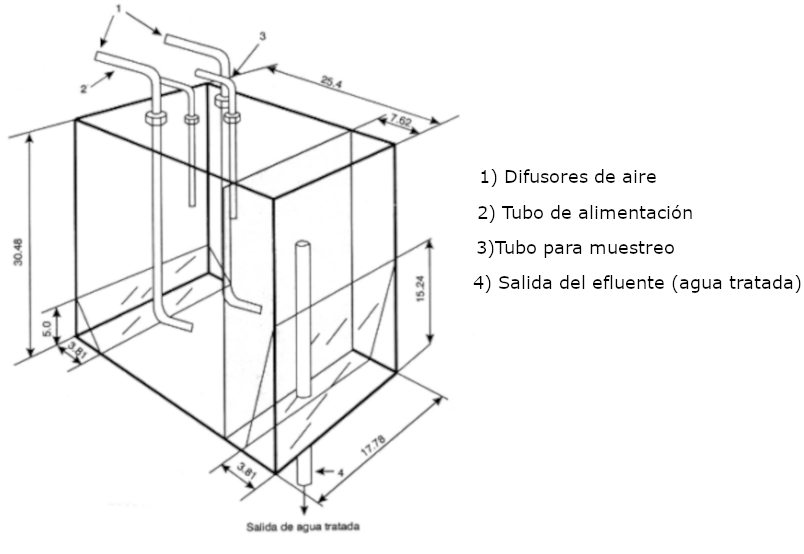
\includegraphics[scale=0.3]{Reactor.png}
	\caption{Biorreactor para la obtención de los parámetros biocinéticos utilizado en el diseño de sistemas de tratamiento de aguas residuales mediante lodos activados}
	\label{fig:reactor}
	\small{Fuente: Martínez (1999)}
\end{figure}
Una vez terminados los reactores, se procederá a preparar el agua residual sintética utilizando como base el \emph{sustrato sintético Nº2} usado por Méndez \textit{et. al.} (2004) \emph{\citep{mendez2004}} descrito en el Cuadro \ref{tab:sustrato}, a su vez, el inoculo se obtendrá de la PTAR municipal de Lagos de Moreno, aclimatandolos por un periodo de 6 días para proseguir con la puesta en marcha de los reactores.
	\begin{table}
	\caption{Composición química del sustrato sintético Nº2}
	\label{tab:sustrato}
	\begin{center}
	\begin{scriptsize}
	\begin{tabular}{|l|c|}
		\hline
		\rowcolor{blanc}
		\multicolumn{1}{|c|}{\textbf{Compuestos}} & \textbf{(mg/L)}\\ \hline
		Gelatina & 34\\
		Almidón & 171\\
		Leche en polvo & 102\\
		Jabón de tocador & 3\\
		MgSO$_{4}$•7H$_{2}$O & 3\\
		KH$_{2}$PO$_{4}$ & 44.5\\
		(NH$_{4}$)$_{2}$SO$_{4}$ & 74.2\\
		NaHCO$_{3}$ & 150\\ \hline
	\end{tabular}
	\end{scriptsize}
	\\ \small{Fuente: Méndez \textit{et. al.} (2004)}
	\end{center}
	\end{table}
\subsubsection*{Determinación de los parámetros cinéticos}
Para la obtención de los parámetros cinéticos se pondrán en marcha los 4 reactores, cada uno con diferente caudal de entrada. Se inocularán con una mezcla del sustrato sintético y los lodos activados ya aclimatados en condiciones de flujo continuo y con aireación constante \citep{delgadillo}. Cada reactor se aireará con ayuda de un compresor de pecera con capacidad de 300 L/Hr. El tiempo en el que los reactores se mantendrán en funcionamiento es aproximadamente de 2 a 4 semanas hasta que el sistema alcanza el equilibrio, realizando toma de muestras y análisis de los constituyentes siguiendo la cronología descrita en el Cuadro \ref{tab:muestreo}.
	\begin{table}[!h]
		\begin{center}
		\caption{Programa de Muestreo}
		\label{tab:muestreo}
		\begin{scriptsize}
			\begin{tabular}{|c|c|c|c|c|}
			\hline
			\rowcolor{blanc}
			Tipo de análisis & Frecuencia & Afluente & \multicolumn{1}{|m{2cm}|}{\centering Licor Mezclado} & Efluente \\
			\hline
			\multicolumn{1}{|m{5cm}|}{\centering DQO, DBO o COT (muestras compuestas; mezclada y sin mezclar)} & \multicolumn{1}{m{3cm}|}{\centering 3 veces por semana} & \multicolumn{1}{m{1.5cm}|}{\centering X} & \multicolumn{1}{m{2cm}|}{\centering } & \multicolumn{1}{m{1.5cm}|}{\centering X} \\
			\hline
			pH & diario & X & X & X \\
			\hline
			Sólidos (SST, (SSV)), VSZ e IVL & 3 veces a la semana & & X & \\
			\hline
			Oxígeno disuelto & diario & & X & \\
			\hline
			VUO & 3 veces a al semana & & X & \\
			\hline
			Observación microscópica & cada semana & & X & \\
			\hline
			\end{tabular}
		\end{scriptsize}
		\small{Fuente: Martínez (1999)}
		\end{center}
	\end{table}
\subsubsection*{Modelado del proceso de lodos activados}
Una vez alcanzado el equilibrio, se procederá a calcular, por el método gráfico de resolución de ecuaciones, las constantes necesarias para el modelado junto con las 4 ecuaciones de estado del sistema. El modelado se realizará usando el comando \emph{ode45} para la solución de las ecuaciones de estado (\emph{ver} Figura \ref{fig:ecuaciones}) con las condiciones de operación del reactor, las condiciones iniciales de operación y el periodo de tiempo en el cual se desarrollará el experimento.

\subsection*{Cronograma}
	\begin{center}
	\begin{footnotesize}
		\begin{tabular}{|p{5.5cm}|p{0.5cm}|p{0.5cm}|p{0.5cm}|p{0.5cm}|p{0.5cm}|p{0.5cm}|p{0.5cm}|p{0.5cm}|p{0.5cm}|p{0.5cm}|p{0.5cm}|}
		\hline
		\rowcolor{blanc}
		Actividades & Ene & Feb & Mar & Abr & May & Jun & Jul & Ago & Sep & Oct & Nov \\ \hline
		\cellcolor{smk} Consulta bibliográfica & \cellcolor{grn}\centering X & \cellcolor{grn}\centering X & \cellcolor{grn}\centering X & \cellcolor{grn}\centering X & & & & & & & \\ \hline
		\cellcolor{smk} Armado de reactores & & \cellcolor{grn}\centering X & & & & & & & & & \\ \hline
		\cellcolor{smk} \scriptsize{Obtención y acondicionamiento de los lodos} & & & \cellcolor{grn}\centering X & & & & & & & & \\ \hline
		\cellcolor{smk} \scriptsize{Determinación de parámetros cinéticos} & & \cellcolor{grn}\centering X & \cellcolor{grn}\centering X & \cellcolor{grn}\centering X & \cellcolor{grn}\centering X & & & & & & \\ \hline
		\cellcolor{smk} Modelado matemático & & & & \cellcolor{grn}\centering X & \cellcolor{grn}\centering X & \cellcolor{grn}\centering X & & & & & \\ \hline
		\cellcolor{smk} Redacción de tesis & & & & & \cellcolor{grn}\centering X & \cellcolor{grn}\centering X & \cellcolor{grn}\centering X & \cellcolor{grn}\centering X & & & \\ \hline
		\cellcolor{smk} \scriptsize{Correcciones y redacción de trabajo final} & & & & & & & & \cellcolor{grn}\centering X & \cellcolor{grn}\centering X & \cellcolor{grn}\centering X & \\ \hline
		\cellcolor{smk} Defensa de tesis & & & & & & & & & & & \cellcolor{grn}\centering X \tabularnewline \hline
		\end{tabular}
	\end{footnotesize}
	\end{center}

\bibliographystyle{plain} 
\bibliography{Bibliografia.bib}
